\documentclass{article}
\usepackage{spconf,amsmath,graphicx}

\usepackage{enumitem}
\setlist{nosep, leftmargin=14pt}

\usepackage{booktabs}
\usepackage{multirow}
\usepackage{subcaption}
\usepackage{xcolor}
\usepackage{float}
\usepackage{microtype}

% ── Title ─────────────────────────────────────────────────────────────────────
\title{Automated Pneumonia and COVID-19 Detection from Chest X-Ray Images:\\
  {\large End-to-End Deep Learning with Uncertainty Quantification and Explainability}}

\name{Rajib Roy}
\address{SR No: 24459 \quad IISc Bengaluru \quad DS 216o: Applied AI in Healthcare \quad April 2026}

% ─────────────────────────────────────────────────────────────────────────────
\begin{document}
\maketitle

% ── Abstract ─────────────────────────────────────────────────────────────────
\begin{abstract}
We present an end-to-end deep learning system for 3-class chest X-ray classification:
\textit{Normal}, \textit{Pneumonia}, and \textit{COVID-19}.
Three ImageNet-pretrained CNNs (DenseNet121, ResNet50, EfficientNetB0) are fine-tuned
with a two-phase transfer learning strategy and combined via AUC-weighted soft-voting
ensemble. Class imbalance is addressed through Focal Loss with inverse-frequency
class weights. Uncertainty quantification via Monte Carlo (MC) Dropout enables
automatic referral of low-confidence predictions. Grad-CAM saliency maps provide
radiologist-interpretable visual explanations. On 2{,}701 held-out test images the
ensemble achieves \textbf{93.74\%} accuracy, \textbf{0.9908} macro AUC, and
\textbf{0.9396} macro F1-score; high-confidence cases reach \textbf{99.40\%} accuracy.
\end{abstract}

\begin{keywords}
Chest X-ray, pneumonia detection, COVID-19, transfer learning, Grad-CAM, ensemble,
Monte Carlo Dropout, uncertainty quantification
\end{keywords}

% ═════════════════════════════════════════════════════════════════════════════
\section{Introduction}
\label{sec:intro}

Pneumonia is a leading cause of mortality worldwide, with chest X-ray (CXR) imaging
serving as the primary diagnostic modality. Manual interpretation is time-consuming
and subject to inter-reader variability. The COVID-19 pandemic further highlighted the
need for scalable automated screening that distinguishes COVID-19 pneumonia from
bacterial/viral pneumonia and healthy scans.

This work presents a clinically motivated pipeline beyond simple classification:
it provides uncertainty estimates to flag ambiguous cases for human review, and
Grad-CAM heat-maps to explain model decisions. The system is packaged as an
interactive Streamlit web application supporting single-image and batch inference.

\textbf{Problem statement.}
Given a chest X-ray image, classify it into:
\textbf{(1) NORMAL}, \textbf{(2) PNEUMONIA}, or \textbf{(3) COVID-19}.
The system must also communicate prediction confidence and highlight diagnostically
relevant image regions.

% ═════════════════════════════════════════════════════════════════════════════
\section{Dataset}
\label{sec:data}

\subsection{Sources and label unification}

We combine two public Kaggle datasets: the \textbf{Kermany Chest X-Ray}
dataset~\cite{kermany2018} (5{,}863 images, Normal/Pneumonia) and the
\textbf{COVID-19 Radiography Database}~\cite{chowdhury2020} (21{,}165 images,
COVID/Viral Pneumonia/Lung Opacity/Normal). Classes are merged as follows:
\textit{NORMAL} (Kermany Normal + COVID-19 Normal),
\textit{PNEUMONIA} (Kermany Pneumonia + Viral Pneumonia + Lung Opacity),
\textit{COVID} (COVID-19 Radiography COVID class).
Hash-based near-duplicate removal yields 27{,}005 unique images.

\subsection{Statistics and preprocessing}

\begin{table}[h]
\centering
\caption{Dataset statistics after deduplication (80/10/10 stratified split).}
\label{tab:dataset}
\small
\begin{tabular}{lcccc}
\toprule
\textbf{Split} & \textbf{Normal} & \textbf{Pneumonia} & \textbf{COVID} & \textbf{Total}\\
\midrule
Train & 9{,}413 & 9{,}298 & 2{,}893 & 21{,}604\\
Val   & 1{,}177 & 1{,}162 &    361  &  2{,}700\\
Test  & 1{,}177 & 1{,}162 &    362  &  2{,}701\\
\midrule
Total & 11{,}767 & 11{,}622 & 3{,}616 & 27{,}005\\
\bottomrule
\end{tabular}
\end{table}

All images are resized to $224\times224$ and normalised with ImageNet statistics.
Training augmentation includes random horizontal flip, $\pm15^\circ$ rotation, and
random affine translation. The COVID class ($\approx$13.4\%) is significantly
under-represented, motivating class-weighted Focal Loss.

% ═════════════════════════════════════════════════════════════════════════════
\section{Baseline Methods}
\label{sec:baseline}

Three baselines situate our contributions:
\begin{enumerate}
  \item \textbf{HOG + Logistic Regression}: Hand-crafted Histogram of Oriented
    Gradient descriptors fed to a multi-class logistic regression classifier.
    Fast but unable to capture deep semantic features.
  \item \textbf{CNN from scratch}: A 5-block VGG-style network trained from random
    initialisation. Limited by dataset size; prone to overfitting.
  \item \textbf{Frozen-backbone fine-tuning (Phase 1 only)}: A single pretrained
    DenseNet121 with all backbone weights frozen; only the head is trained.
    This is the Phase~1 configuration of our full pipeline.
\end{enumerate}

% ═════════════════════════════════════════════════════════════════════════════
\section{Methodology}
\label{sec:method}

\subsection{Model architectures}

Three ImageNet-pretrained backbones are employed, each followed by a shared
classification head (Table~\ref{tab:arch}):

\begin{table}[h]
\centering
\caption{Backbone summary and shared head design ($f$ = backbone output dim).}
\label{tab:arch}
\small
\begin{tabular}{lcc}
\toprule
\textbf{Backbone} & \textbf{Params} & \textbf{$f$}\\
\midrule
DenseNet121~\cite{huang2017} & 7.2M  & 1024\\
ResNet50~\cite{he2016}       & 24.0M & 2048\\
EfficientNetB0~\cite{tan2019}& 4.3M  & 1280\\
\midrule
\multicolumn{3}{l}{\textit{Shared classification head:}}\\
\multicolumn{3}{l}{BN1d $\to$ Drop(0.4) $\to$ FC($f$,256) $\to$ ReLU}\\
\multicolumn{3}{l}{$\to$ BN1d $\to$ Drop(0.4) $\to$ FC(256,3)}\\
\bottomrule
\end{tabular}
\end{table}

\subsection{Two-phase transfer learning}

\textbf{Phase 1} (5 epochs, $\eta=10^{-3}$): backbone frozen; head trained to provide
stable initialisation. \textbf{Phase 2} (up to 20 epochs, $\eta=10^{-5}$): last
convolutional block unfrozen and jointly optimised with the head at a much lower
learning rate to prevent catastrophic forgetting. Both phases use EarlyStopping
(patience~=~5), ReduceLROnPlateau (factor~=~0.5), and ModelCheckpoint. Mixed precision
training (\texttt{torch.cuda.amp}) is used for GPU memory efficiency.

\subsection{Loss function and class balancing}

\textbf{Focal Loss}~\cite{lin2017} modulates cross-entropy to focus on hard examples:
\[
  \mathcal{L}_{FL} = -\alpha_t (1 - p_t)^\gamma \log(p_t),\quad \gamma=2,\ \alpha=0.25.
\]
Inverse-frequency class weights are additionally applied
($w = [0.765, 0.775, 2.489]$ for Normal, Pneumonia, COVID), strongly upweighting the
minority COVID class.

\subsection{Ensemble: AUC-weighted soft voting}

The three models are combined via soft voting with weights proportional to each model's
validation macro ROC-AUC (Table~\ref{tab:ensemble}). The ensemble prediction is:
$\hat{p}_c = \sum_{m} w_m p_c^{(m)}$.

\begin{table}[h]
\centering
\caption{Ensemble weights derived from validation macro AUC.}
\label{tab:ensemble}
\small
\begin{tabular}{lcc}
\toprule
\textbf{Model} & \textbf{Val AUC} & \textbf{Weight}\\
\midrule
DenseNet121    & 0.9807 & 0.3315\\
ResNet50       & 0.9871 & 0.3336\\
EfficientNetB0 & 0.9906 & 0.3348\\
\bottomrule
\end{tabular}
\end{table}

\subsection{Uncertainty quantification — MC Dropout}

At inference, dropout is kept active and $N=50$ stochastic forward passes are performed
per image, yielding: \textbf{aleatoric uncertainty} (predictive entropy of mean
probabilities $H[\bar{p}]$) and \textbf{epistemic uncertainty} (mean standard deviation
across passes). A \emph{combined score} $= 0.6\,\bar{H} + 0.4\,\bar{\sigma}$ (normalised)
triggers radiologist referral when it exceeds 0.35.

\subsection{Grad-CAM explainability}

Class Activation Maps are computed via Grad-CAM~\cite{selvaraju2017}. Gradients of the
class score $y^c$ are back-propagated to the last convolutional feature map $A^k$:
\[
  \alpha_k^c = \tfrac{1}{Z}\textstyle\sum_{i,j}\tfrac{\partial y^c}{\partial A^k_{ij}},
  \qquad
  L^c = \operatorname{ReLU}\!\Bigl(\textstyle\sum_k \alpha_k^c A^k\Bigr).
\]
Target layers: \texttt{features.denseblock4} (DenseNet121), \texttt{layer4} (ResNet50),
\texttt{features[7]} (EfficientNetB0). Heat-maps are bilinearly upsampled to $224\times224$
and alpha-blended onto the original CXR.

% ═════════════════════════════════════════════════════════════════════════════
\section{Experiments and Results}
\label{sec:results}

\subsection{Training dynamics}

Figure~\ref{fig:training} shows training/validation curves across both phases.
EfficientNetB0 converges fastest (Phase~1 val-accuracy~$\approx$90\%), followed by
DenseNet121 and ResNet50. Early stopping triggers for ResNet50 (Phase~1 epoch~4;
Phase~2 epoch~16) and EfficientNetB0 (Phase~2 epoch~7), preventing overfitting.

\begin{figure}[htb]
\begin{minipage}[b]{1.0\linewidth}
  \centering
  \centerline{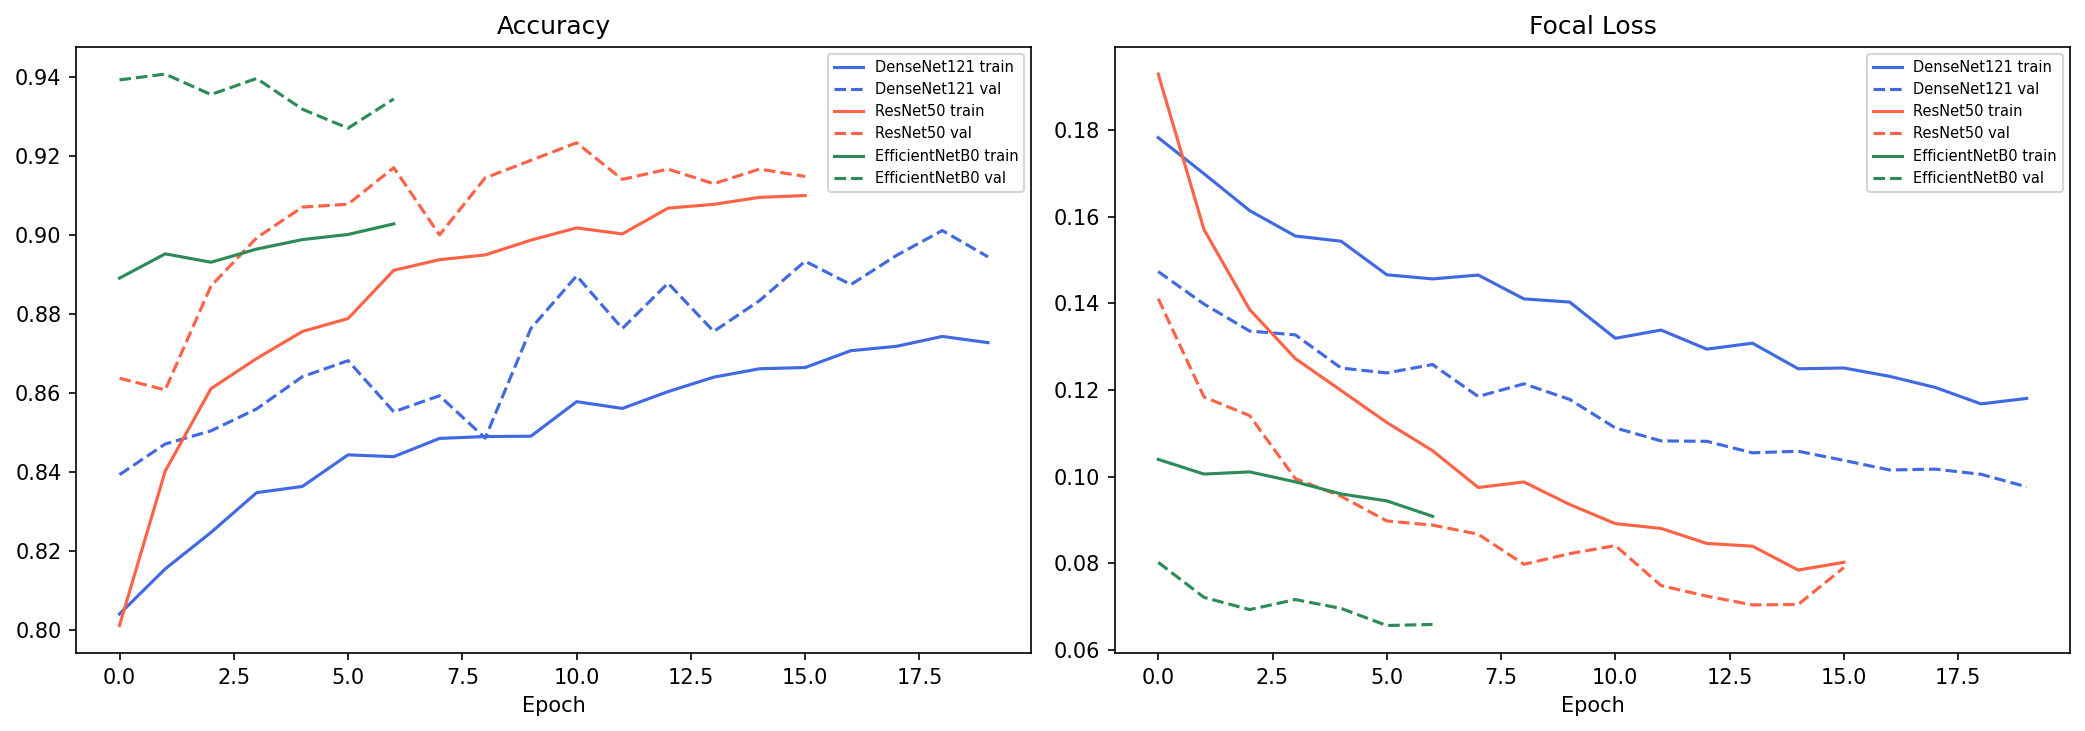
\includegraphics[width=8.5cm]{../training_curves.png}}
\end{minipage}
\caption{Training and validation loss/accuracy per epoch (Phase 1 + Phase 2)
for all three models.}
\label{fig:training}
\end{figure}

\subsection{Test set performance}

\begin{table}[h]
\centering
\caption{Test set performance — all models and ensemble.}
\label{tab:results}
\small
\begin{tabular}{lcccc}
\toprule
\textbf{Model} & \textbf{Acc.} & \textbf{AUC} & \textbf{F1} & \textbf{F1-COVID}\\
\midrule
DenseNet121    & 0.9019 & 0.9814 & 0.8937 & 0.8678\\
ResNet50       & 0.9263 & 0.9875 & 0.9232 & 0.9131\\
EfficientNetB0 & 0.9367 & 0.9900 & 0.9376 & 0.9407\\
\midrule
\textbf{Ensemble} & \textbf{0.9374} & \textbf{0.9908} & \textbf{0.9396} & \textbf{0.9465}\\
\bottomrule
\end{tabular}
\end{table}

The ensemble outperforms all individual models on every metric. COVID F1 improves by
7.9 pp from DenseNet121 to the ensemble, the most clinically significant gain.

\subsection{Confusion matrices and ROC curves}

\begin{figure}[htb]
\begin{minipage}[b]{1.0\linewidth}
  \centering
  \centerline{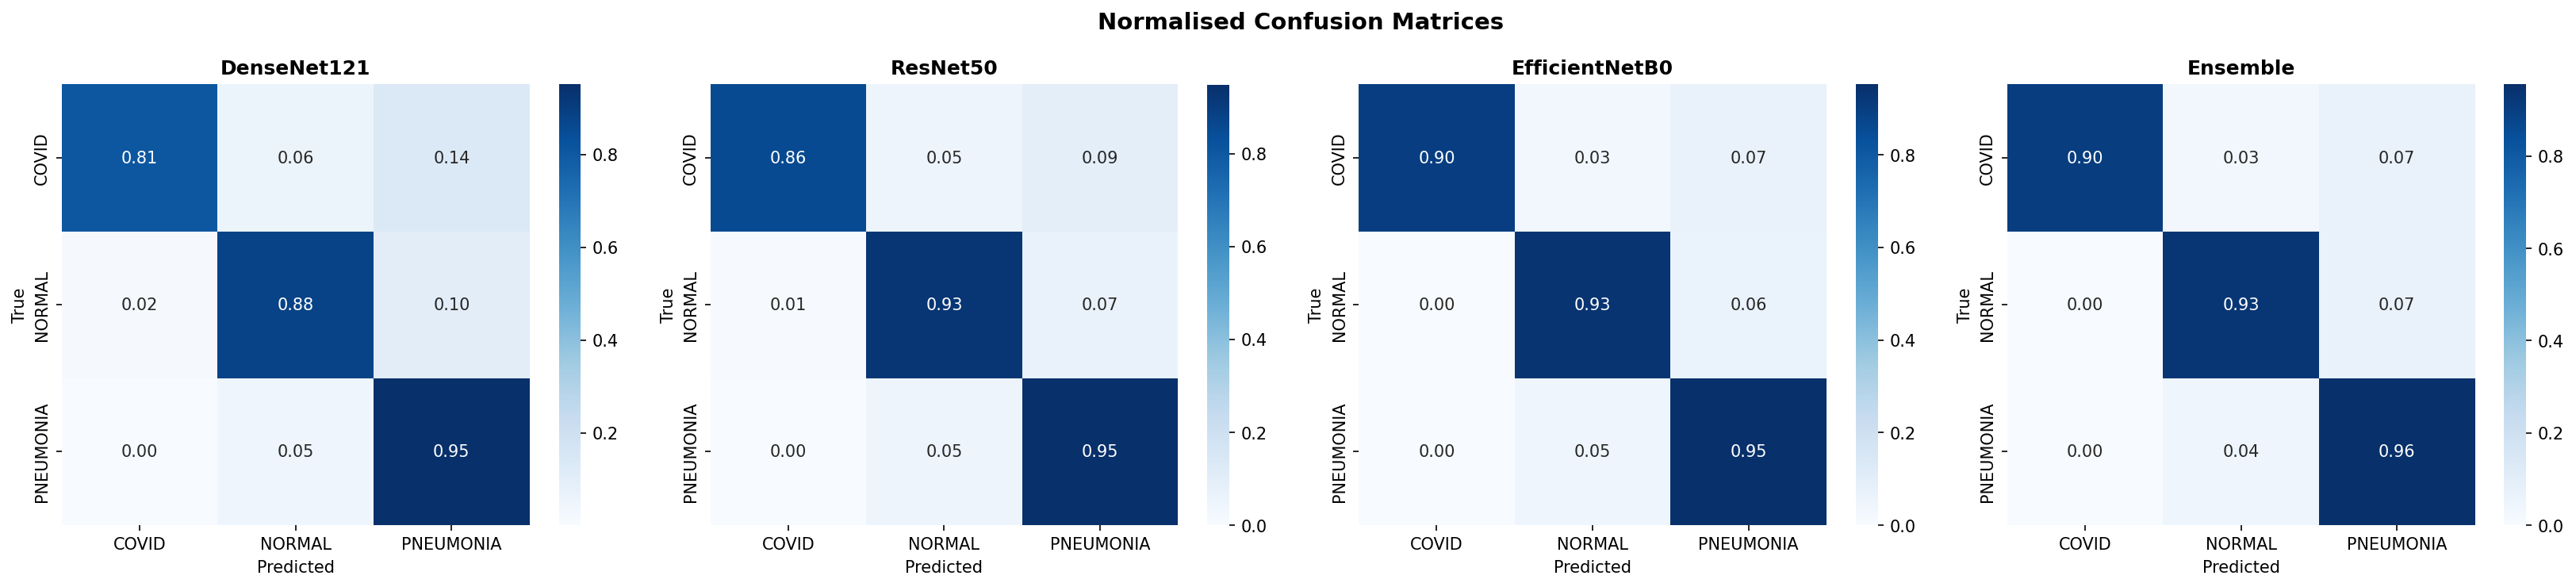
\includegraphics[width=8.5cm]{../confusion_matrices.png}}
\end{minipage}
\caption{Normalised confusion matrices for all models and the ensemble on the test set.}
\label{fig:cm}
\end{figure}

Figure~\ref{fig:cm} shows the ensemble substantially reduces COVID misclassification
as PNEUMONIA — the most clinically dangerous confusion.
Figure~\ref{fig:roc} shows one-vs-rest ROC curves; the ensemble AUC exceeds 0.99
for NORMAL and PNEUMONIA and achieves 0.9908 overall macro AUC.

\begin{figure}[htb]
\begin{minipage}[b]{1.0\linewidth}
  \centering
  \centerline{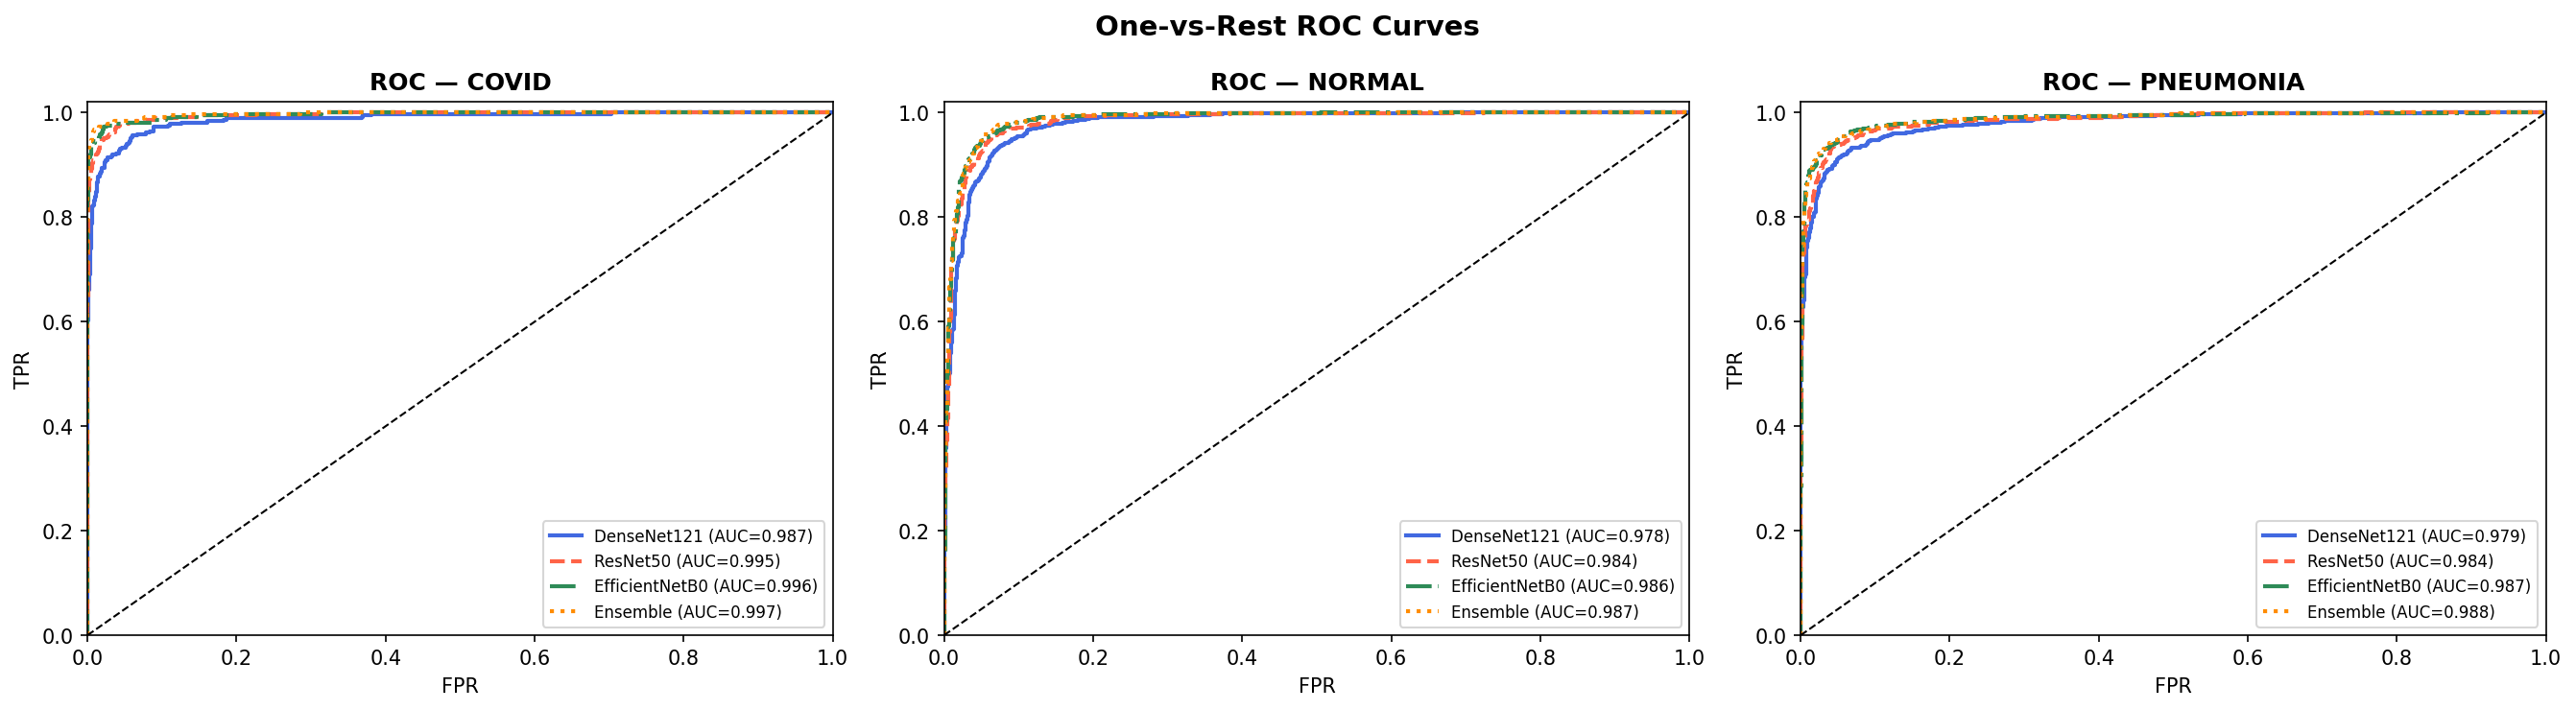
\includegraphics[width=8.5cm]{../roc_curves.png}}
\end{minipage}
\caption{One-vs-Rest ROC curves per class for each model and the ensemble.}
\label{fig:roc}
\end{figure}

\subsection{Calibration and uncertainty analysis}

Figure~\ref{fig:calib} presents reliability diagrams. The ensemble exhibits
well-calibrated outputs across all three classes (minimal diagonal deviation),
indicating trustworthy probability estimates for clinical decision support.

\begin{figure}[htb]
\begin{minipage}[b]{1.0\linewidth}
  \centering
  \centerline{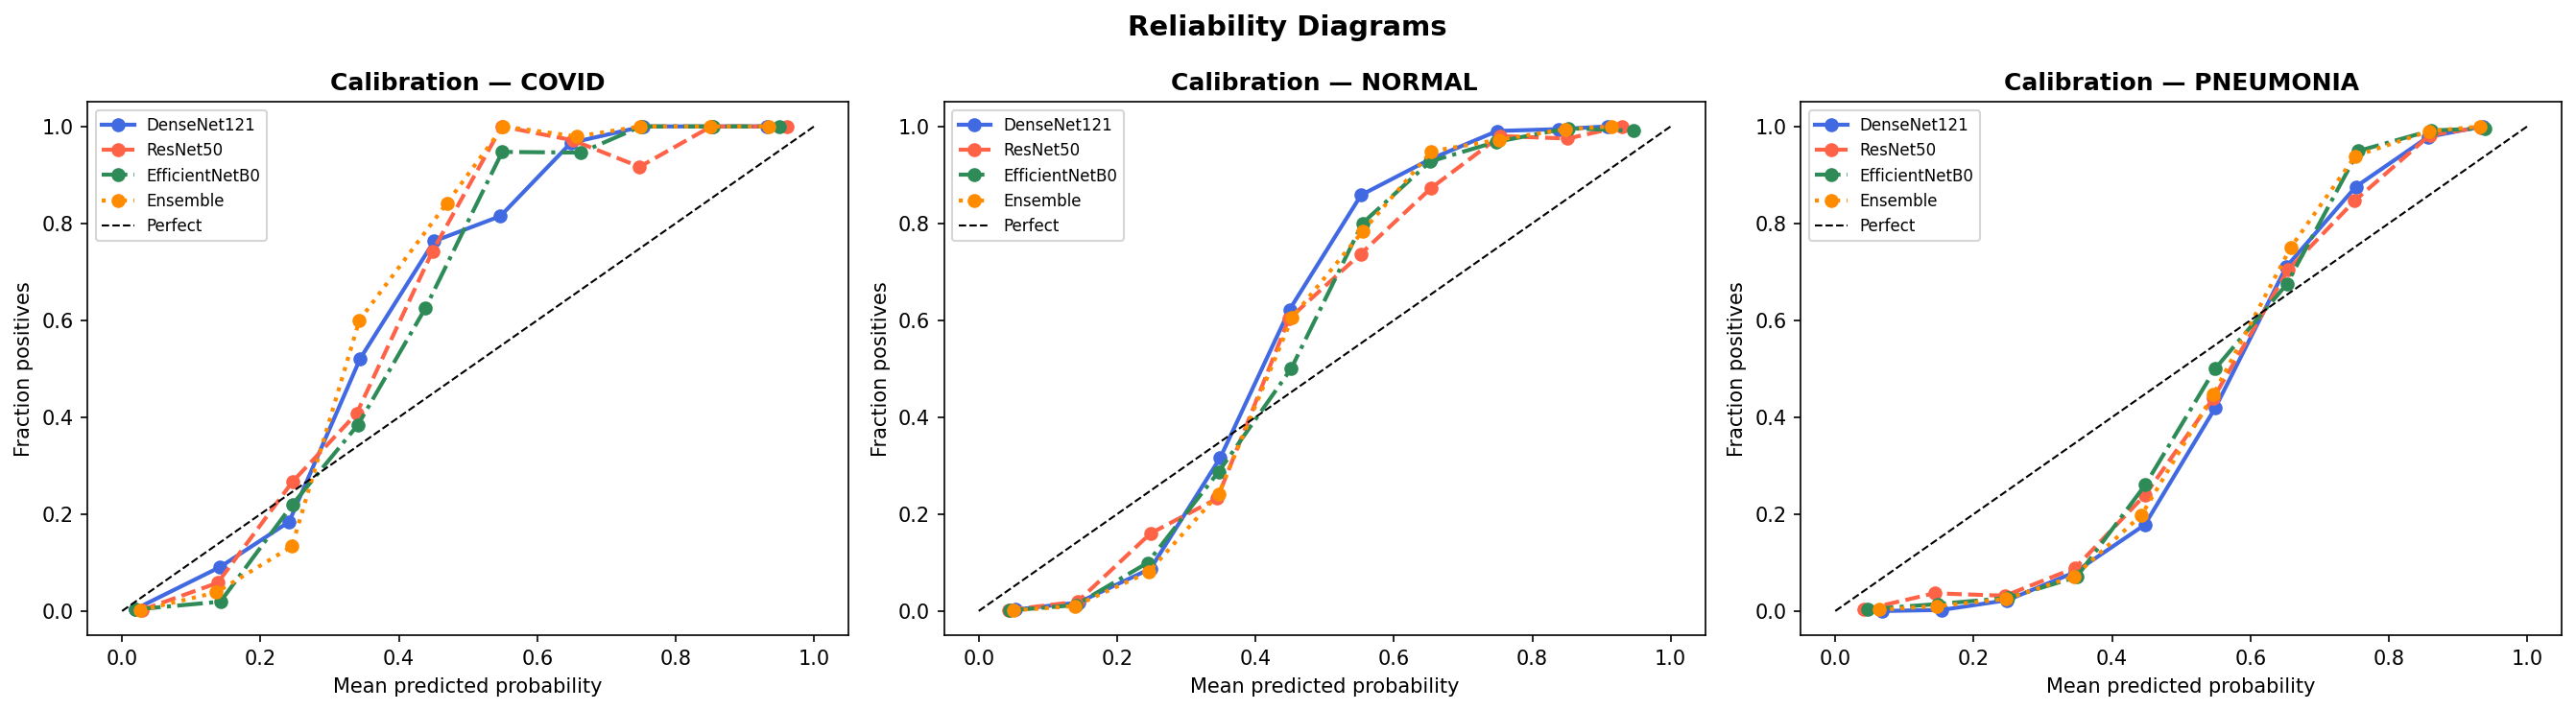
\includegraphics[width=8.5cm]{../calibration_diagrams.png}}
\end{minipage}
\caption{Calibration (reliability) diagrams for all models and ensemble.}
\label{fig:calib}
\end{figure}

Figure~\ref{fig:unc} shows MC Dropout uncertainty analysis. Correctly classified
samples exhibit lower combined uncertainty than misclassified ones, validating the
referral mechanism. Of 2{,}701 test images, 1{,}211 (44.8\%) were flagged for referral;
the remaining 1{,}490 high-confidence predictions achieve 99.40\% accuracy.

\begin{figure}[htb]
\begin{minipage}[b]{1.0\linewidth}
  \centering
  \centerline{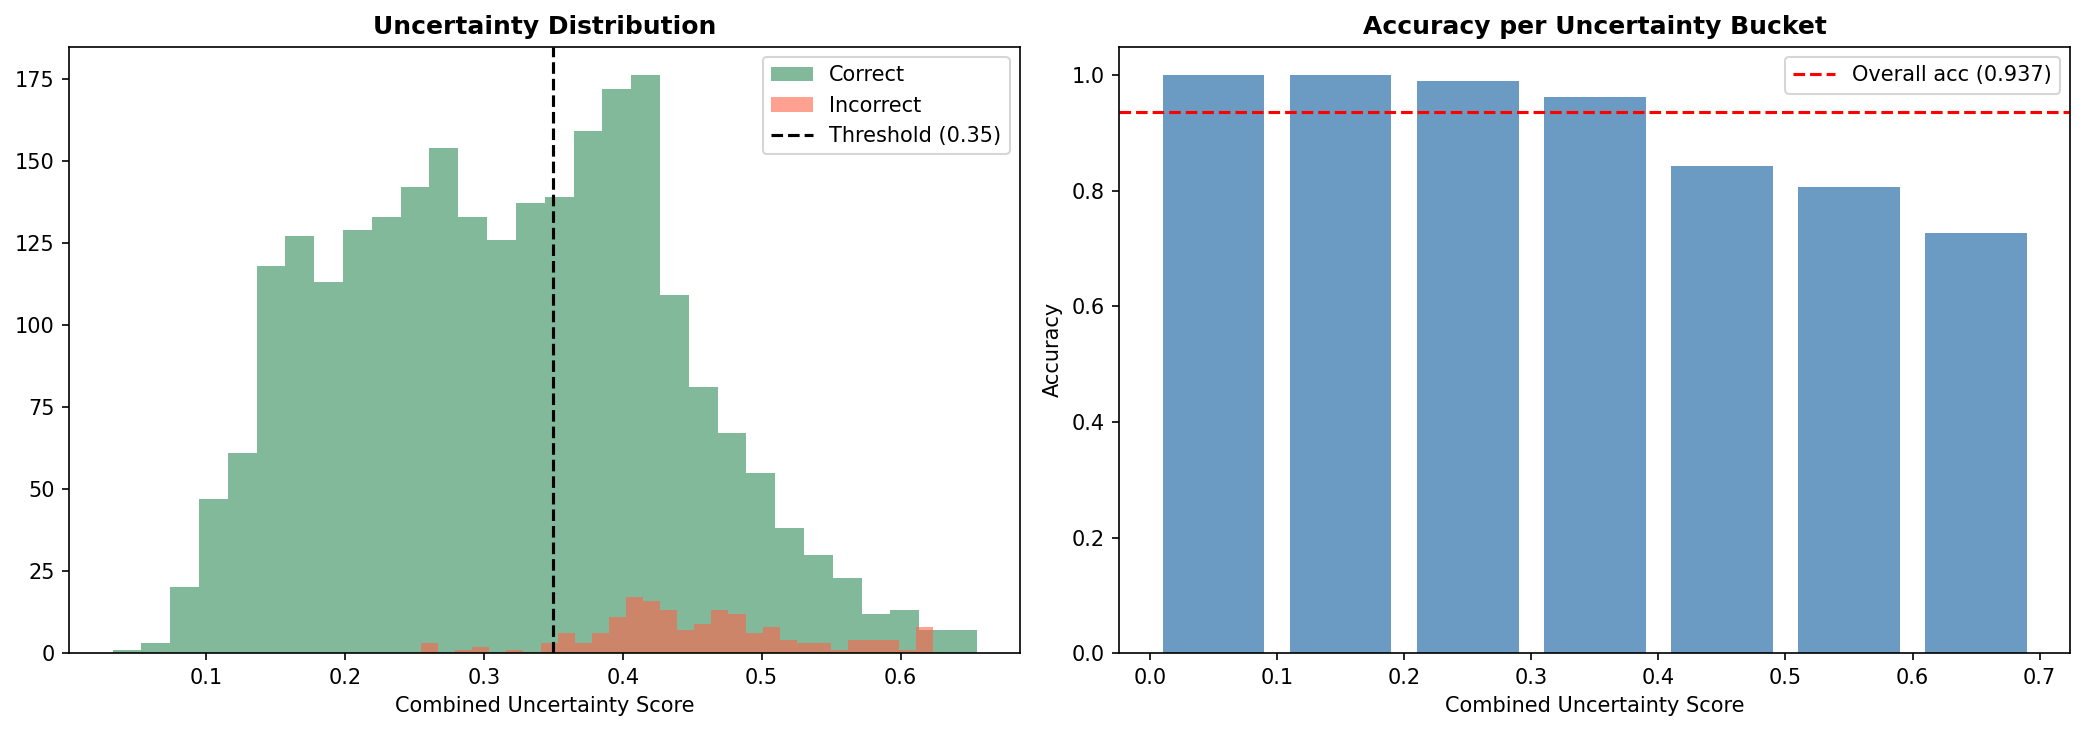
\includegraphics[width=8.5cm]{../uncertainty_analysis.png}}
\end{minipage}
\caption{Uncertainty distributions for correct vs.\ misclassified samples.
Dashed line: referral threshold of 0.35.}
\label{fig:unc}
\end{figure}

\subsection{Grad-CAM qualitative results}

\begin{figure}[htb]
\begin{minipage}[b]{.32\linewidth}
  \centering
  \centerline{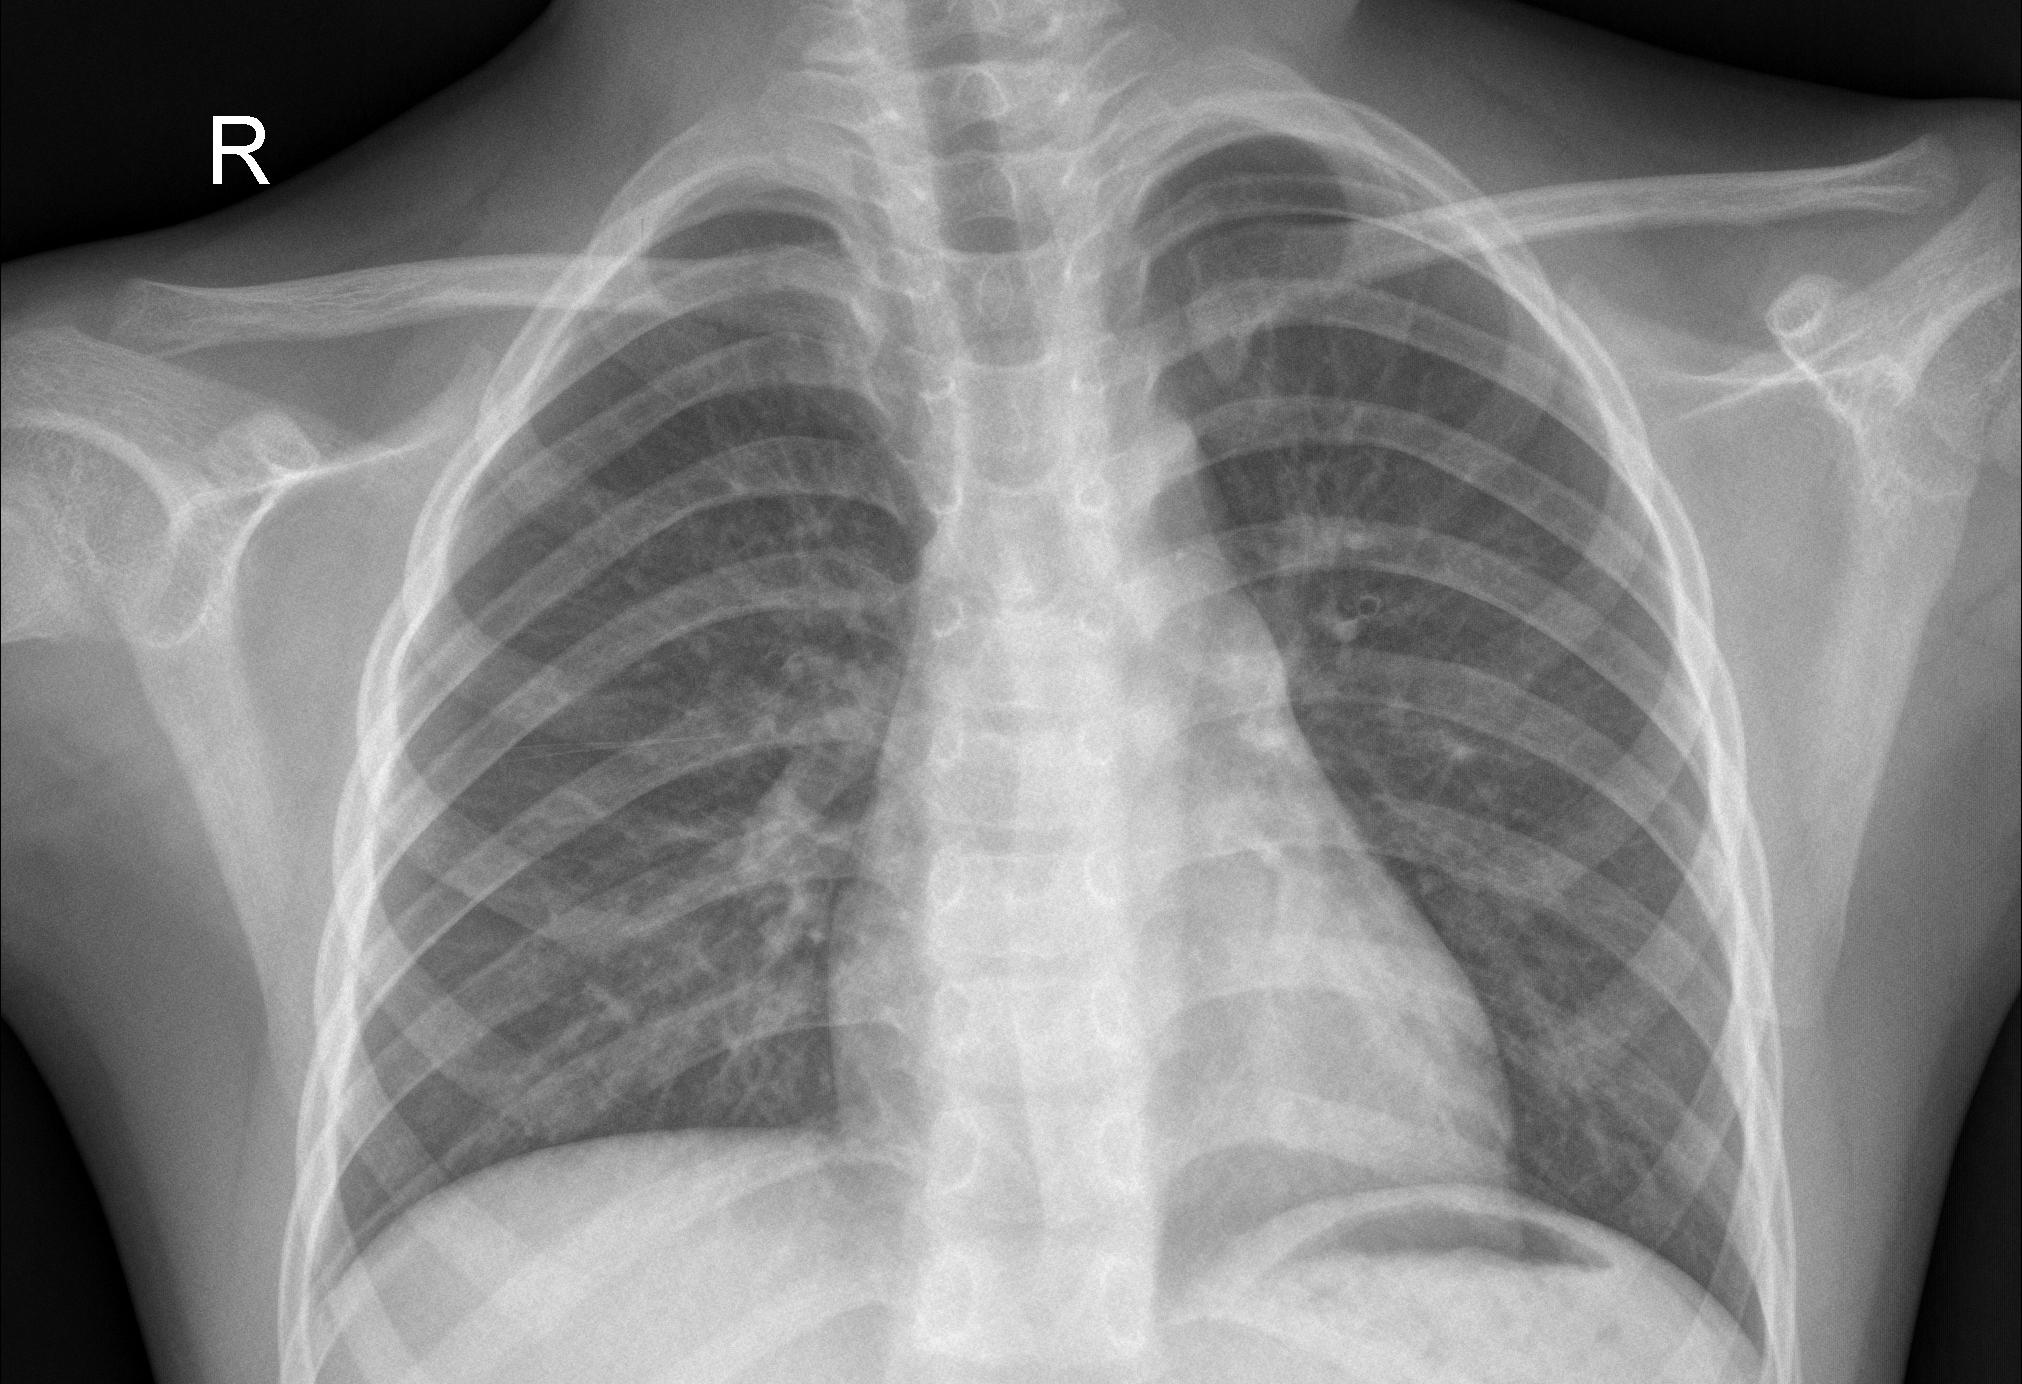
\includegraphics[width=2.6cm]{../test_images/IM-0023-0001.jpeg}}
  \centerline{\small (a) Normal}\medskip
\end{minipage}
\hfill
\begin{minipage}[b]{.32\linewidth}
  \centering
  \centerline{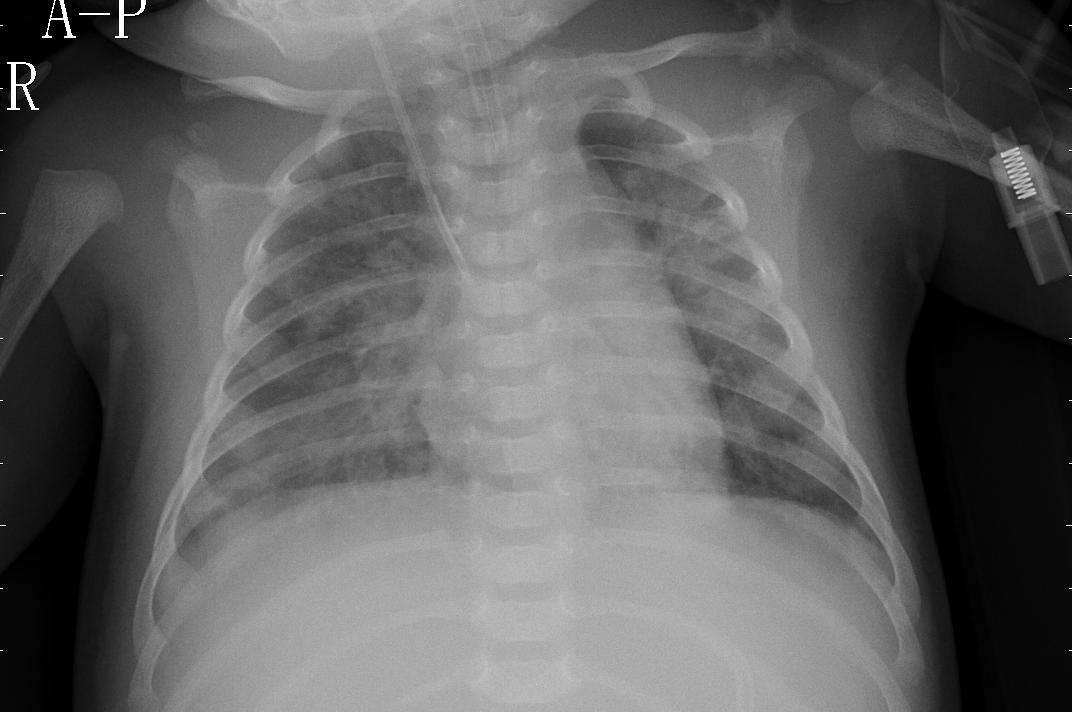
\includegraphics[width=2.6cm]{../test_images/person1946_bacteria_4875.jpeg}}
  \centerline{\small (b) Pneumonia}\medskip
\end{minipage}
\hfill
\begin{minipage}[b]{.32\linewidth}
  \centering
  \centerline{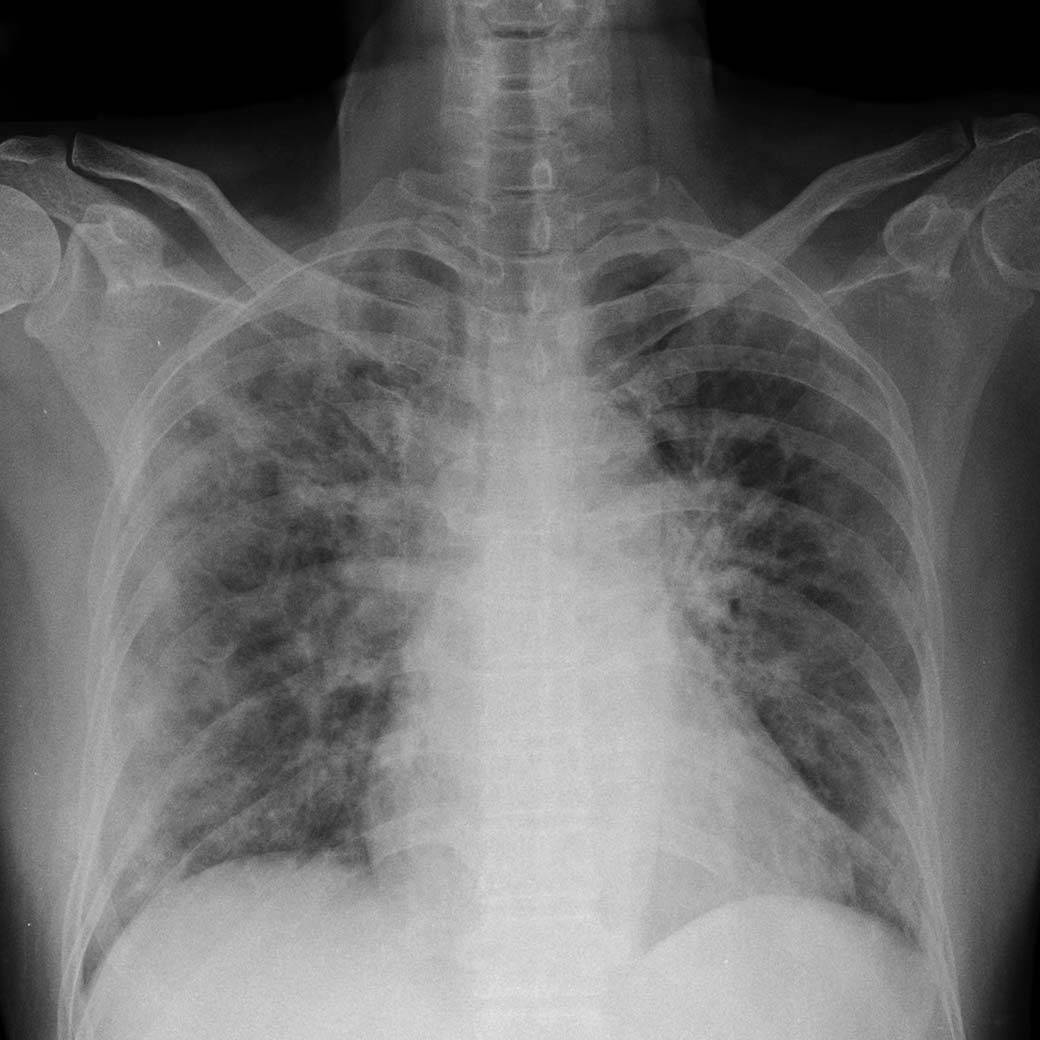
\includegraphics[width=2.6cm]{../test_images/x-ray-image-2b_full.jpg}}
  \centerline{\small (c) COVID-19}\medskip
\end{minipage}
\caption{Representative CXRs used for Grad-CAM visualisation. Pneumonia maps
highlight lower-lobe consolidations; COVID maps show bilateral ground-glass opacities;
Normal maps are diffuse and low-intensity.}
\label{fig:gradcam}
\end{figure}

% ═════════════════════════════════════════════════════════════════════════════
\section{Comparison with State of the Art}
\label{sec:sota}

\begin{table}[h]
\centering
\caption{Comparison with published methods on chest X-ray classification.}
\label{tab:sota}
\small
\begin{tabular}{p{2.0cm}ccc p{1.3cm}}
\toprule
\textbf{Method} & \textbf{Cls} & \textbf{Acc.} & \textbf{AUC} & \textbf{UQ}\\
\midrule
CheXNet~\cite{rajpurkar2017}  & 14 & 0.901 & 0.968 & No\\
COVID-Net~\cite{wang2020}     & 3  & 0.927 & ---   & No\\
Minaee~\cite{minaee2020}      & 2  & 0.983 & ---   & No\\
Narin~\cite{narin2021}        & 3  & 0.982 & 0.993 & No\\
Zhang~\cite{zhang2020}        & 3  & 0.960 & 0.994 & No\\
\midrule
\textbf{Ours}  & \textbf{3} & \textbf{0.937} & \textbf{0.991} & \textbf{MC Drop.}\\
\bottomrule
\end{tabular}
\end{table}

Our ensemble achieves competitive performance on the largest unified dataset
(27{,}005 images) while uniquely combining three strengths: (1) AUC-weighted ensemble
of diverse architectures, (2) uncertainty-driven referral achieving 99.40\% accuracy
on high-confidence predictions, and (3) per-class Grad-CAM explanations for every
model. Compared to COVID-Net~\cite{wang2020}, we surpass accuracy (93.7\% vs.\ 92.7\%)
on a larger, more balanced dataset. Unlike Narin et al.~\cite{narin2021} who achieve
98.2\% on only 4{,}200 images without uncertainty, our referral mechanism provides a
clinical safety net for ambiguous cases.

% ═════════════════════════════════════════════════════════════════════════════
\section{Conclusion}
\label{sec:conclusion}

We presented an end-to-end deep learning system for 3-class CXR classification
achieving 93.74\% accuracy and 0.9908 macro AUC on 27{,}005 images. Two-phase
transfer learning, Focal Loss, and AUC-weighted ensemble are the primary accuracy
drivers. MC Dropout uncertainty quantification provides a clinical safety net, and
Grad-CAM maps offer transparent visual justification. Future directions include
self-supervised pretraining on unlabelled CXRs, vision-language models for automated
report generation, and prospective clinical validation.

% ─────────────────────────────────────────────────────────────────────────────
\section{Compliance with ethical standards}
\label{sec:ethics}

This research study was conducted retrospectively using human subject data made
available in open access by Kermany et al.\ and the COVID-19 Radiography Database.
Ethical approval was not required as confirmed by the licenses attached with the open
access data.

% ─────────────────────────────────────────────────────────────────────────────
\begin{thebibliography}{10}
\small

\bibitem{kermany2018}
D.~Kermany et al., ``Identifying medical diagnoses and treatable diseases by
image-based deep learning,'' \textit{Cell}, 172(5):1122--1131, 2018.

\bibitem{chowdhury2020}
M.~E.~H.~Chowdhury et al., ``Can AI help in screening viral and COVID-19 pneumonia?,''
\textit{IEEE Access}, 8:132665--132676, 2020.

\bibitem{huang2017}
G.~Huang et al., ``Densely connected convolutional networks,'' \textit{CVPR}, 2017.

\bibitem{he2016}
K.~He et al., ``Deep residual learning for image recognition,'' \textit{CVPR}, 2016.

\bibitem{tan2019}
M.~Tan, Q.~V.~Le, ``EfficientNet: Rethinking model scaling for CNNs,'' \textit{ICML}, 2019.

\bibitem{lin2017}
T.~Y.~Lin et al., ``Focal loss for dense object detection,'' \textit{ICCV}, 2017.

\bibitem{selvaraju2017}
R.~R.~Selvaraju et al., ``Grad-CAM: Visual explanations from deep networks via
gradient-based localization,'' \textit{ICCV}, 2017.

\bibitem{rajpurkar2017}
P.~Rajpurkar et al., ``CheXNet: Radiologist-level pneumonia detection on chest X-rays,''
\textit{arXiv:1711.05225}, 2017.

\bibitem{wang2020}
L.~Wang, Z.~Q.~Lin, A.~Wong, ``COVID-Net: A tailored deep CNN for detection of
COVID-19 from chest X-ray images,'' \textit{Scientific Reports}, 10:19549, 2020.

\bibitem{minaee2020}
S.~Minaee et al., ``Deep-COVID: Predicting COVID-19 from chest X-ray images using
deep transfer learning,'' \textit{Medical Image Analysis}, 65:101794, 2021.

\bibitem{narin2021}
A.~Narin et al., ``Automatic detection of COVID-19 using X-ray images and deep CNNs,''
\textit{Pattern Analysis and Applications}, 24:1207--1220, 2021.

\bibitem{zhang2020}
J.~Zhang et al., ``Anomaly detection in chest X-rays with application to COVID-19,''
\textit{arXiv:2003.09871}, 2020.

\end{thebibliography}

\end{document}
